%
% File Name: scratch.tex
% Author:    Aditya Ramesh
% Date:      12/21/2014
% Contact:   _@adityaramesh.com
%

%\subsection{Activation Functions and Feature Learning}
%
%So far in our discussion, we have avoided making specific choices for the
%activation function $u_{kj}$ associated with unit $(k, j)$. This is because the
%choice of activation function depends largely on the kind of problem we are
%trying to solve, the location of $L_k$ in the network, and the role of the
%features we are trying to extract using $\sigma_k$. Choosing the best activation
%functions for a particular problem can also involve a certain degree of
%experimentation. We present some general guidelines based on current practices
%in the literature.
%
%Neural networks have successfully been used to solve many kinds of tasks in
%machine learning. These tasks include classification, regression, density
%estimation (using mixture density networks), dimensionality reduction (using
%autoencoders), and similarity learning (using siamese networks). Despite the
%diversity of the tasks solved, the principles used to construct the network
%architectures to solve them are largely the same. One of the most important
%principles that underlies the success of neural networks is that of hierarchial
%feature learning.
%
%A \emph{feature} is a ``simple'' quantity derived from the input that is
%designed to identify one or more of the input's salient characteristics. For
%example, suppose that we wish to identify whether a given black and white image
%contains a human face. One potential feature is the difference between the sum
%of intensities of the pixels in the left half of the image and that of the right
%half of the image. In neural networks, a feature is a subset of activations that
%become large when a given pattern is present in the input. This is a result of
%the weights and biases of the network being attuned to presence the pattern.
%
%The success of neural networks in image recognition and acoustic modeling has
%been attributed to their ability to learn a \emph{hierarchy} of features. In
%these applications, the location of a layer $L_k$ in the network determines the
%relative scale of the patterns in the input captured by the features. In some
%sense, the lowest layers of the network ``zoom in'' to the input to characterize
%low-level, local details, while the highest layers of the network ``zoom out''
%to characterize overarching, global patterns (see
%Figure~\ref{fig:cnn_features}).  It is plausible that this phenomenon can occur,
%since each $\sigma_k$ synthesizes the information from layers $L_0, \ldots, L_{k
%- 1}$ to produce $z_k$.
%
%Activation functions measure the richness of features in the input. Typically,
%an activation function ``squashes'' the activation to a small range, such as
%$[-1, 1]$ or $[0, 1]$. Near zero, activation functions behave linearly, and away
%from zero, activation functions saturate to minimum and maximum values. The
%exception to these rules is the identity function, which is used for regression.
%The two most common activation functions other than the identity are the
%scaled hyperbolic tangent and linear threshold functions (see
%Figure~\ref{fig:activation_plots}).

% TODO: revise the previous paragraph; the characterization of act func is
% inaccurate.

\pagebreak
\thispagestyle{empty}
\newgeometry{top = 0in, left = 0in, right = 0in}
\begin{figure}
\centering
\resizebox{\textwidth}{!}{%
	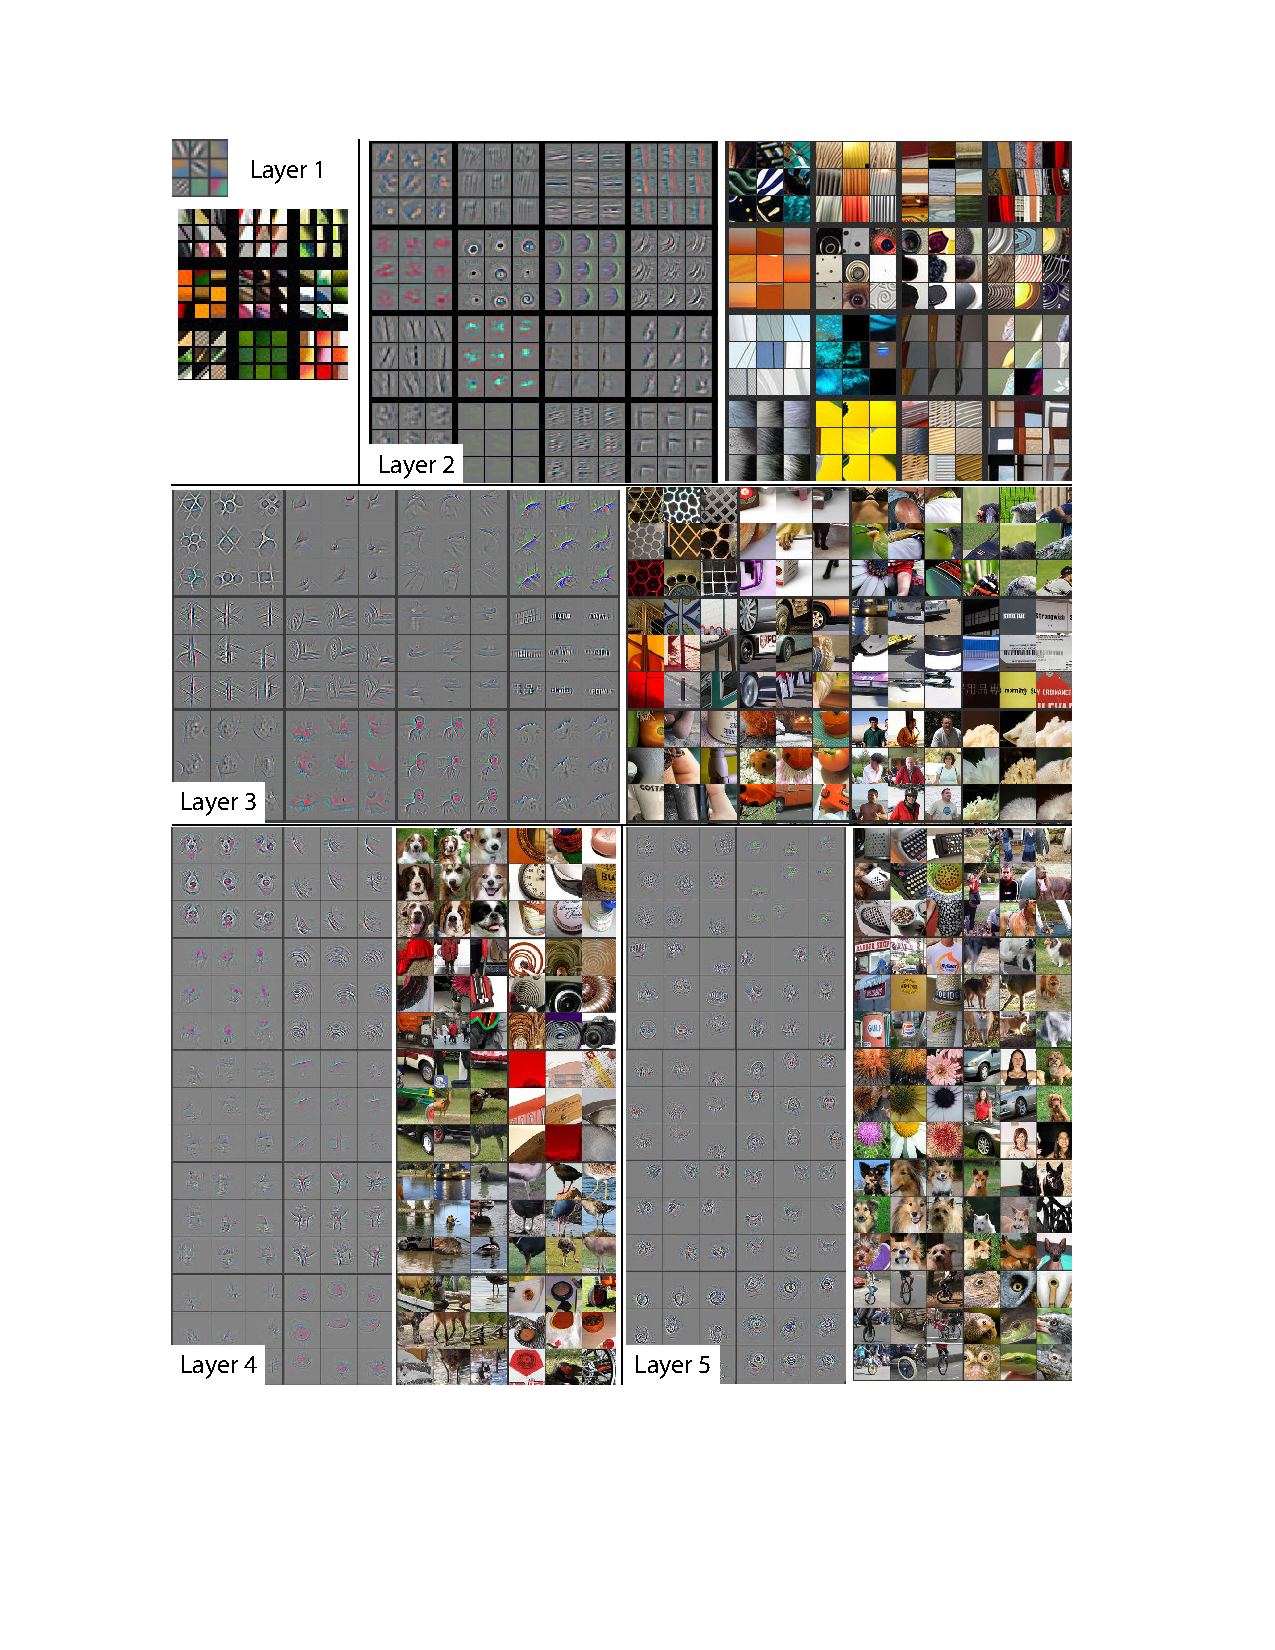
\includegraphics[trim = 0in 1in 0in 0in]{graphics/cnn_features.pdf}
}
\begin{minipage}[c]{\textwidth - 2in}
\caption{Visualization of the hierarchy of features in a fully-trained
convolutional network for image classification. For each of the first five
layers of the network, a selection of the highest activations in the layer is
shown alongside the corresponding input images. Note that in general,
visualizing features in a meaningful way is very difficult. TODO: reference
paper!\label{fig:cnn_features}}
\end{minipage}
\end{figure}
\pagebreak
\restoregeometry

%% SECTION BREAK
%
%
% TODO: make the notation the same as in the previous figure.
%\begin{figure}[t]
%\scriptsize\centering
%\begin{tikzpicture}
%\node[lightstyle, minimum size=20] (a1) at (-2,0) {$x_{k1}$};
%\node[lightstyle, minimum size=20] (a2) at (-1,0) {$x_{k2}$};
%\node[lightstyle, minimum size=20] (a3) at (0,0) {$x_{k3}$};
%\node[lightstyle, minimum size=20] (a4) at (1,0) {$x_{k4}$};
%\node[lightstyle, minimum size=20] (a5) at (2,0) {$x_{k5}$};
%
%\node[darkstyle, minimum size=20] (b1) at (-2,1.5) {$z_{11}$};
%\node[darkstyle, minimum size=20] (b2) at (-1,1.5) {$z_{12}$};
%\node[darkstyle, minimum size=20] (b3) at (0,1.5) {$z_{13}$};
%\node[darkstyle, minimum size=20] (b4) at (1,1.5) {$z_{14}$};
%\node[darkstyle, minimum size=20] (b5) at (2,1.5) {$z_{15}$};
%
%\node[lightstyle, minimum size=20] (c1) at (-2,3) {$\hat{y}_{k1}$};
%\node[lightstyle, minimum size=20] (c2) at (-1,3) {$\hat{y}_{k2}$};
%\node[lightstyle, minimum size=20] (c3) at (0,3) {$\hat{y}_{k3}$};
%\node[lightstyle, minimum size=20] (c4) at (1,3) {$\hat{y}_{k4}$};
%\node[lightstyle, minimum size=20] (c5) at (2,3) {$\hat{y}_{k5}$};
%
%\node[lightstyle, minimum size=20] (y) at (4,0) {$y_k$};
%
%\draw (-2.5,4.2) rectangle (4.5,5.2) node[fitting node] (error) {};
%\draw (1,4.7) node {Error};
%
%\node at (0,-0.75) {$x_k$};
%\node at (-3.5,0) {\scriptsize Input layer};
%\node at (-3.5,1.5) {\scriptsize Hidden layer};
%\node at (-3.5,3) {\scriptsize Output layer};
%
%\draw[-stealth] (a1)--(b1);
%\draw[-stealth] (a1)--(b2);
%\draw[-stealth] (a2)--(b1);
%\draw[-stealth] (a2)--(b2);
%\draw[-stealth] (a2)--(b3);
%\draw[-stealth] (a3)--(b2);
%\draw[-stealth] (a3)--(b3);
%\draw[-stealth] (a3)--(b4);
%\draw[-stealth] (a4)--(b3);
%\draw[-stealth] (a4)--(b4);
%\draw[-stealth] (a4)--(b5);
%\draw[-stealth] (a5)--(b4);
%\draw[-stealth] (a5)--(b5);
%
%\draw[-stealth] (b1)--(c1);
%\draw[-stealth] (b1)--(c2);
%\draw[-stealth] (b2)--(c1);
%\draw[-stealth] (b2)--(c2);
%\draw[-stealth] (b2)--(c3);
%\draw[-stealth] (b3)--(c2);
%\draw[-stealth] (b3)--(c3);
%\draw[-stealth] (b3)--(c4);
%\draw[-stealth] (b4)--(c3);
%\draw[-stealth] (b4)--(c4);
%\draw[-stealth] (b4)--(c5);
%\draw[-stealth] (b5)--(c4);
%\draw[-stealth] (b5)--(c5);
%
%\path
%	let
%		\p1 = (c1),
%		\p2 = (c2),
%		\p3 = (c3),
%		\p4 = (c4),
%		\p5 = (c5),
%		\p6 = (y),
%		\p7 = (error.south)
%	in
%		node (d1) at (\x1,\y7+3) {}
%		node (d2) at (\x2,\y7+3) {}
%		node (d3) at (\x3,\y7+3) {}
%		node (d4) at (\x4,\y7+3) {}
%		node (d5) at (\x5,\y7+3) {}
%		node (d6) at (\x6,\y7+3) {};
%
%\draw[-stealth] (c1)--(d1);
%\draw[-stealth] (c2)--(d2);
%\draw[-stealth] (c3)--(d3);
%\draw[-stealth] (c4)--(d4);
%\draw[-stealth] (c5)--(d5);
%\draw[-stealth] (y)--(d6);
%\end{tikzpicture}
%
%\caption{A visualization of how the $k$th training data point $(x_k,y_k)$ is fed
%into a two-layer neural network, where $x_k \in \reals{m}$ and $y_k \in
%\reals{n}$. Because the input layer simply reflects the input vector $x_k$, it
%is not included in the total layer count. The outputs of the units in the output
%layer collectively determine $\hat{y}_k$, the prediction of the neural network for
%$x_n$. The error module, which computes the discrepancy between the predicted
%output $\hat{y}_k$ and the target output $y_k$, is only used during
%training.\label{fig:neural_network}}
%\end{figure}
%\subsection{Learning}
%
%The training data is typically partitioned into three disjoint sets: the
%training set, the validation set, and the test set. The training set is used to
%calibrate the weights of the neural network in order to improve performance on
%the validation set. Until the error on the validation is less than a given
%threshold, we repeatedly iterate through the training set to calibrate the
%weights, and measure the subsequent performance on the validation set. Each one
%of these cycles through the training and validation sets is called an
%\emph{epoch}. If, after a certain number of epochs, the validation error is
%still above the given threshold, then we abandon the training procedure. After
%the training procedure, the test set is used to provide a final assessment of
%the network's performance. Of course, it is important that no information
%derived from either the validation set or the test set influences the training
%of the network.
%
%In machine learning, the objective is not to minimize the error on the training
%set, but rather to achieve good generalization to the test set. Good performance
%on the training set but poor performance on the validation set, or good
%performance on the validation set but poor performance on the test set, are both
%potential indicators of overfitting. In overfitting, the weights of the model
%are tuned to small fluctuations between samples in the training set, rather than
%to the overarching mapping between the input and target vectors that we would
%like to approximate. Various approaches may be taken to combat
%overfitting \cite{mlpr_book}.
%
%During the training phase, each input vector from the training set is presented
%to the network. Each unit in the input layer of the network simply reflects the
%corresponding component of the current input vector $x_n$. Units in
%successive layers of the network then recursively compute their activations and
%outputs in accordance with Equations~\ref{eq:activation} and~\ref{eq:output}.
%This process is called \emph{forward propagation}. The outputs of the units in
%the output layer of the network are then collectively regarded as the network's
%prediction $y_n$ for the input vector $x_n$. The error function
%$e(y,t,w,b)$, which is only used during training,
%measures the discrepancy between the predicted output $y_n$ and the target
%output $t_n$. The process of training can then be viewed as an
%unconstrained minimization problem, in which we seek to minimize the error
%function over the samples in the training set. The choice of error function
%plays an vital role in guiding the network during training.
%
%\subsection{Configuration}
%
%\begin{figure}
%\centering
%\begin{tikzpicture}
%\begin{axis}[
%	xmin=-4,
%	xmax=4,
%	xlabel=$x$,
%	ylabel=$y$
%]
%\addplot[mark=none, samples=100] {1.7159 * tanh(2 * x / 3)};
%\end{axis}
%\end{tikzpicture}
%\caption{Plot of the logistic sigmoid function $y = a\tanh(bx)$, where $a =
%1.7159$ and $b = 2/3$.\label{fig:logistic_sigmoid}}
%\end{figure}
%
%We have carried on our discussion of neural networks without mentioning specific
%choices for the activation or error functions. We now briefly outline some
%common choices for these functions in order to accomplish various tasks.
%Typically, the same activation function is chosen for all units in the same
%layer. By far the most common choice of activation function for hidden units is
%the logistic sigmoid, which is shown in Figure~\ref{fig:logistic_sigmoid}. The
%logistic sigmoid is an odd function that is approximately linear near the
%origin, and approaches constant asymptotes as $x \to \pm\infty$. The constants
%$a$ and $b$ in the logistic sigmoid are chosen so that, when the inputs are
%decorrelated, the variance of the outputs will be close to one
%\cite{efficient_backprop}. This has been shown to accelerate learning in neural
%networks.
%
%When binary coding is used for the target vector $t_n$ in classification
%tasks, the values are typically chosen to be 1 or -1. These values correspond to
%the critical points of the second derivative of the logistic sigmoid given in
%Figure~\ref{fig:logistic_sigmoid}. The target values are then within the
%sigmoid's useful range, rather than at its asymptotes. This avoids numerical
%instabilities, since weights will not be forced to assume large values in order
%for the sigmoid to output the target values. Setting the target values within
%the sigmoid's useful range also enables us to interpret the proximity of the
%sigmoid's output to the nearest target value as a measure of confidence of the
%network's classification.
%
%While the logistic sigmoid is a common choice for the activation function of
%hidden units, several other functions can also be used. The choice of activation
%function for hidden units is largely open to experimentation. In contrast, the
%choice of the output activation and error functions is often motivated by the
%task and specific features of the problem being addressed.
%
%Assume that we are given a data set $D = \{ (x_1, t_1), \ldots,
%(x_N, t_N) \}$. If we assume an explicit representation for the
%posterior distribution $p(t_n \given x_n, w, b)$ of the
%target vector with respect to the input, weights, and biases of the network,
%then we are led to a canonical error function. This canonical error function is
%obtained by maximizing the likelihood function for the network over all of the
%instances in $D$. If we assume that the instances in $D$ are identically
%distributed, then given $x_n$, $w$ and $b$, we know that
%$t_n$ is conditionally independent of $\{ x_i \}_{i \neq n}$. Using
%the chain rule, we can write the likelihood function as
%\begin{equation}
%	p(t_1, \ldots, t_n \given x_1, \ldots, x_n,
%	w, b) = \prod_{n = 1}^N p(t_n \given x_n,
%	w, b).
%	\label{eq:likelihood_function}
%\end{equation}
%Maximizing Equation \ref{eq:likelihood_function} is equivalent to minimizing its
%negative logarithm, which is given by
%\begin{align*}
%	-\ln{p(t_1, \ldots, t_n \given x_1, \ldots, x_n,
%	w, b)} &= -\sum_{n = 1}^N \ln{p(t_n \given x_n,
%	w, b)}.
%\end{align*}
%We now define the per-sample error function $e(y,t,w,b)$
%by
%\[
%	e(y_n, t_n, w, b) =
%	-\ln{p(t_n \given x_n, w, b)},
%\]
%and the error function $E(w,b)$ evaluated over the entire training
%data set by
%\[
%	E(w,b) =
%	\sum_{n = 1}^N e(y_n, t_n, w, b).
%\]
TODO: define the per-sample and cumulative error functions on the same line.
%In practice, $e$ may exclude some constants from $-\ln{p(t_n \given
%x_n, w, b)}$ that do not affect the minimization process.
%Table~\ref{tab:output_activations} shows some common choices for the output
%activation function; Table~\ref{tab:posterior_distributions} shows common
%choices for the posterior distribution $p(t_n \given x_n, w,
%b)$, and the resulting error functions.
TODO: mention that by selecting a posterior distribution, we are led to a
corresponding choice of loss function.
%
%\begin{table}[t]
%\centering
%\captionof{table}{Common choices for the output activation function
%\cite{mlpr_book}.}
%\label{tab:output_activations}
%\begin{tabular}{ll}
%\toprule
%Task & $y_n(a_n)$ \\
%\midrule
%Regression & Identity \\
%Unary classification & Logistic Sigmoid \\
%Multiclass classification & Softmax \\
%\bottomrule
%\end{tabular}
%\bigskip
%
%\captionof{table}{Common choices for the posterior distribution
%\cite{mlpr_book}.}
%\label{tab:posterior_distributions}
%\begin{tabular}{llll}
%\toprule
%Task &
%$p(t_n \given x_n, w, b)$ &
%$E(w, b)$ \\
%\midrule
%Regression & Gaussian & Sum-of-squares \\
%Unary classification & Bernoulli & Unary cross-entropy \\
%Multiclass classification & Categorical & Multiclass cross-entropy \\
%\bottomrule
%\end{tabular}
%\end{table}
%
%\subsection{Optimization}
%
%We mentioned earlier that the process of training the network can be viewed as
%an unconstrained minimization problem, in which we wish to minimize the error
%function $E(w, b)$ over the samples in the training data set. The
%\emph{steepest descent} method has shown great success in the training of neural
%networks (\cite{efficient_backprop}, \cite{large_datasets_slides}). To motivate
%the derivation of steepest descent and discuss its properties, we appeal to the
%field of numerical optimization.
%
%The following discussion of the steepest descent method is adapted from the one
%given in \cite{numerical_optimization_notes}. We temporarily drop the boldface
%notation for vectors, because there is no possibility of confusing vectors with
%scalars. Let $D$ be an open convex subset of $\reals{n}$, and suppose that $f :
%D \to \reals{1}$ is a continuously-differentiable function. We define $g$ and
%$H$ to be the gradient and Hessian of $f$, respectively. The \emph{Taylor-series
%linear model} of $f$ near the base point $\bar{x} \in D$ is given by
%\begin{equation}
%	l(x) \coloneqq f(\bar{x}) + \trans{g(\bar{x})} (x - \bar{x}).
%	\label{eq:linear_model}
%\end{equation}
%
%Equation~\ref{eq:linear_model} suggests a line search procedure in which the
%$k$th search direction $p_k$ is chosen to achieve the greatest reduction in
%$l(x_k)$, where $x_k$ is the current iterate. Define $f_k = f(x_k)$ and $g_k
%= g(x_k)$. Clearly, the greatest reduction in $l(x_k)$ is achieved by
%minimizing the inner product $\trans{g_k}p_k$. However, $p_k$ can be chosen to
%make the inner product $\trans{g_k}p_k$ arbitrarily large and negative, so we
%impose the norm constraint $\norm{p_k} = \gamma$. To minimize $\trans{g_k}p_k$
%subject to the norm constraint, we apply the Cauchy-Schwartz inequality. The
%Cauchy-Schwartz inequality states that, for any two vectors $y$ and $z$, we have
%$\trans{y}z \geq -\norm{y}\norm{z}$, with equality only when $y$ is a positive
%multiple of $-z$. It follows that $\trans{g_k}p_k$ is minimized when
%\[
%	p_k = -\frac{\gamma}{\norm{g_k}} g_k,
%\]
%so that $p_k$ is the normalized \emph{negative gradient vector}
%\cite{numerical_optimization_notes}. Choosing $\gamma = \norm{g_k}$ leads to the
%particularly simple search direction
%\[
%	p_k = -g_k.
%\]
%Hence, the update rule for steepest descent becomes
%\begin{align}
%	x_{k + 1} &= x_k + \alpha_k p_k \notag\\
%	&= x_k - \alpha_k g_k, \label{eq:steepest_descent_update}
%\end{align}
%where the step size $\alpha_k$ is chosen by a line search procedure.
%
%If the step size $\alpha_k$ is chosen such that the Armijo or strong Wolfe
%conditions are satisfied (e.g. by backtracking line search), then steepest
%descent is guaranteed to converge to a minimizer of $f$. Unfortunately, the
%convergence of steepest descent is linear in the best case, and the convergence
%rate is bounded by an asymptotic error constant that grows closer to unity as
%distance between the largest and smallest eigenvalues of $H$ increases
%\cite{numerical_optimization_notes}. In other words, as $H$ becomes increasingly
%ill-conditioned, the convergence of steepest descent can become arbitrarily
%slow. This result will inform us as we apply steepest descent to train neural
%networks.
%
%\section{Stability}
%
%\subsection{The System}
%
%To apply steepest descent to train neural networks, we minimize the error
%function over the samples in the training data set. The following discussion
%only mentions the weights of the network and not the biases, because the results
%that we derive for the weights can be extended analogously to the biases. Using
%steepest descent to minimize the error function $E(w, b)$ would
%require one pass through the entire training data set to perform one update to
%the weights which corresponds to Equation~\ref{eq:steepest_descent_update}. The
%step $p_k$ is taken as the average of the gradient across all of the samples in
%the training data set. Defining
%\[
%	g_n =
%	\nabla_{w} e(y_n, t_n, w_k, b_k),
%\]
%we have
%\[
%	p_k = -\frac{1}{N} \sum_{n = 1}^N g_n,
%\]
%and
%\begin{equation}
%	w_{k + 1} = w_k + \alpha_k p_k.
%	\label{eq:gradient_descent_update}
%\end{equation}
%In the machine learning literature, the step size $\alpha_k$ is called the
%\emph{learning rate}. The gradient and Hessian of a neural network can both be
%computed using a technique for recursively computing partial derivatives called
%\emph{backpropagation} (\cite{mlpr_book}, \cite{efficient_backprop}). Using
%backpropagation, computing the gradient requires $O(W)$ operations, and
%computing the full Hessian requires $O(W^2)$ operations, where $W$ is the number
%of weights in the network.
%
%\emph{Batch gradient descent}, which performs the update given by
%Equation~\ref{eq:gradient_descent_update} after every $M$ samples, can converge
%much more rapidly than the update over the entire training data set. The extreme
%case corresponding to $M = 1$, called \emph{stochastic gradient descent}, has
%been shown to be much more effective than batch methods at training neural
%networks \cite{efficient_backprop}.
%
%The following explanation for why stochastic gradient descent can be more
%effective than batch gradient descent is paraphrased from
%\cite{efficient_backprop}. Imagine a training data set of size 1000 that is
%inadvertently composed of 10 identical copies of a set with 100 samples.
%Averaging the gradient over all 1000 data points gives the same result as
%computing the gradient based on just the first 100. A batch update over the
%entire data set would compute the same quantity 10 times before performing one
%update. On the other hand, stochastic gradient descent would see a full epoch as
%10 iterations through a training data set of size 100. While identical copies
%are a rare occurrence in practice, we often encounter clusters of patterns that
%are very similar.
%
%We have not yet mentioned how we are to choose the learning rate $\alpha_k$
%during the optimization process. Based on our discussion, the most obvious
%choice would be to use a line search procedure that satisfies Armijo or strong
%Wolfe conditions, such as the backtracking line search. However, we are left
%with the task of selecting the Armijo parameter $\eta_s$ and the contraction
%factor $\gamma$ for the line search, where $0 < \eta_s \leq 1/2$ and $0 < \gamma
%< 1$. The choices for these constants are usually made arbitrarily, and poor
%choices will lead to unnecessarily small step sizes or an excessive number of
%iterations in the backtracking line search procedure. Fortunately, there is a
%natural choice for the optimal learning parameter that we can derive using
%stability theory.
%
%We now desire to view the update rule given by
%Equation~\ref{eq:gradient_descent_update} as a discrete dynamical system.
%Although the step size $p_k$ depends on the current batch of $M$ samples,
%we make the assumption that the iteration order of the samples does not
%significantly change the dynamics of the system. Given a batch size $M$, we now
%consider the discrete dynamical system given by
%\[
%	w_{k + 1} = f(w_k),
%	\label{eq:discrete_dynamical_system}
%\]
%where
%\begin{equation}
%	f(w_k) = w_k - \frac{\alpha_k}{M} \sum_{n = 1}^M g_n.
%	\label{eq:update_function}
%\end{equation}
%
%\subsection{Fixed Points}
%
%To find the fixed points of Equation~\ref{eq:discrete_dynamical_system}, we
%solve the equation
%\[
%	f(w_k) - w_k = 0,
%\]
%from which we deduce that
%\[
%	\sum_{n = 1}^N g_n = 0.
%\]
%This agrees with the result that the gradient of a continuously-differentiable
%function must be zero at an unconstrained minimizer.
%
%To determine the stability of the fixed points, we construct the linearization
%of Equation~\ref{eq:discrete_dynamical_system}. Computing the Jacobian of $f$,
%we have
%\begin{align*}
%	J(w) &= \nabla_{w} f(w) \\
%	&= 1 - \frac{\alpha_k}{M} \sum_{n = 1}^M H_n,
%\end{align*}
%where $H_n$ is given by
%\[
%	H_n =
%	\nabla_{w}^2 e(y_n, t_n, w_k, b_k).
%\]
%Now, let $w^*$ be a fixed point. Stability theory tells us that
%$w^*$ will be stable if $\spectrum{\complexes{1}}(J(w^*))
%\subset (-1, 1)$. Recall that adding $\lambda I$ to a matrix has the effect of
%shifting all of the eigenvalues by $\lambda$, where $\lambda \in \reals{1}$.
%Define
%\[
%	H \coloneqq \sum_{n = 1}^M H_n.
%\]
%We can formulate bounds on the learning rate $\alpha_k$ by solving the equation
%\[
%	\left| 1 - \frac{\alpha_k}{M} \lambda_{max} \right| < 1,
%	\label{eq:spectrum_bounds}
%\]
%where $\lambda_{max}$ is the eigenvalue of $H$ having the largest
%magnitude. Solving Equation~\ref{eq:spectrum_bounds} for $\alpha_k$ yields the
%solution interval
%\[
%	0 < \alpha_k < \frac{2M}{\lambda_{max}}.
%	\label{eq:learning_rate_bounds}
%\]
%
%It remains to determine which value of $\alpha_k$ to select from the interval
%given by Equation~\ref{eq:learning_rate_bounds}. Recall that the convergence
%rate of steepest descent is bounded by an asymptotic error constant that grows
%closer to unity as the distance between the largest and smallest eigenvalues of
%$H$ increases. Therefore, we should aim to reduce the spread of the
%eigenvalues of $H$ as much as possible. The best we can do using a scalar
%learning rate is to shift $\lambda_{max}$ to zero. The value of $\alpha_k$ that
%achieves this is obtained by solving the equation
%\[
%	1 - \frac{a_k}{M} \lambda_{max} = 0,
%\]
%which is satisfied by
%\[
%	\alpha^* = \frac{M}{\lambda_{max}}.
%\]
%
%The optimal scalar learning rate $\alpha^*$ scales all of the components of the
%gradient in order to ensure stability of the fixed point $w^*$. A more
%general result regarding the shifting of eigenvalues states that, if a scalar
%$\lambda \in \reals{1}$ is added to the $i$th diagonal element of a matrix, then
%the corresponding eigenvalue is also shifted by $\lambda$. Consequently, we can
%further improve convergence by allowing $\alpha_k$ to be a vector, so that
%Equation~\ref{eq:update_function} now becomes
%\[
%	f(w_k) =
%	w_k - M^{-1} \trans{\alpha}_k \sum_{n = 1}^M g_n.
%\]
%The optimal value of the $i$th component $\alpha_i$ of $\alpha_k$ can be
%determined analogously to the case where $\alpha_k$ is a scalar. Hence, we have
%\[
%	\alpha_i = \frac{M}{\lambda_i},
%\]
%where $\lambda_i$ is the eigenvalue corresponding to the $i$th diagonal of
%$H$.
%
%In practice, iterative methods such as the power method are used to approximate
%$\lambda_{max}$ \cite{efficient_backprop}. While using separate learning rates
%for each weight is still advisable, computing the full Hessian is prohibitively
%expensive, and is not done in practice. Fortunately, approximations based on
%$\lambda_{max}$ tend to work very well in practice, because the distribution of
%the eigenvalues of the $H$ typically has a large peak at eigenvalues of
%very small magnitude, a smaller peak at eigenvalues of small magnitude, and a
%few outliers having very large magnitude \cite{efficient_backprop}. These few
%outliers dominate the optimization process.
%
%\subsection{Trajectories}
%
%Consider a two-layer neural network, such as the one given in
%Figure~\ref{fig:neural_network}. If we negate the weights directed toward a unit
%$i$ in the hidden layer, along with the unit's bias, then we negate the
%activation $a_i$. If we assume that $u_i$ is an odd function, such as the
%logistic sigmoid, then we have $u_i(-a_i) = -u_i(a_i)$. If we also negate the
%weights directed away from unit $i$, then the output of the network will be
%unchanged. Hence, each unit $i$ in the hidden layer has two equivalent weight
%configurations that leave the output of the network invariant. The total number
%of these \emph{sign-flip symmetries} is given by $2^M$, where $M$ is the number
%of units in the hidden layer.
%
%If we assume that the same activation function is used for all units in the
%hidden layer, then there are additional symmetries to be considered. We can swap
%the weights directed toward and away from any hidden unit $i$, along with the
%unit's bias, with those of another hidden unit $j$, while leaving the output of
%the network invariant. The total number of these \emph{interchange symmetries}
%is given by $M!$. In total, there are $M! \, 2^M$ symmetries for a given
%configuration $w$ and $b$ of the weights and biases of the network
%\cite{mlpr_book}. This number grows much larger as the numbers of units and
%layers in the network are increased. It is no surprise that one of the greatest
%challenges in training neural networks is avoiding running into local minima.
%
%A natural question to ask is whether the trajectory resulting from a small
%perturbation of the initial condition $w_0$ will converge to a different
%minimizer under Equation~\ref{eq:update_function}. One approach to answering
%this question is to examine the Lyapunov spectrum of the orbit of $w_0$.
%As we mentioned earlier, there are typically only a handful of eigenvalues of
%large magnitude that dominate the optimization process. If the Lyapunov numbers
%corresponding to these eigenvalues are greater than one, then the behavior of
%iterates near $w_0$ may be chaotic. Hence, we would expect the trajectory
%of $w_0$ to be sensitive to small perturbations. On the other hand, if the
%Lyapunov numbers corresponding to the large eigenvalues are small, then we would
%expect the orbits of other initial conditions near $w_0$ to converge to
%the same minimizer.
%
%Suppose that we use the optimal scalar learning rate with
%Equation~\ref{eq:update_function}. Then the Jacobian is given by
%\begin{align*}
%	J(w)
%	&= 1 - \frac{1}{\lambda_{max}} \sum_{n = 1}^M H_n \\
%	&= 1 - \frac{1}{\lambda_{max}} H.
%\end{align*}
%Using the optimal learning rate has the effect of transforming the eigenvalues
%of $J$ so that the maximal Lyapunov number is less than one. Hence, we can
%think of the scaling the Hessian by $\lambda_{max}^{-1}$ as a preventative
%measure against chaotic behavior of the trajectory of $w_0$.
%
%\section{Conclusion}
%
%We have introduced the concept of a neural network as a graphical template for
%constructing nonlinear functions to perform classification and regression tasks.
%The steepest descent method, which has traditionally only been used as a
%fallback when more sophisticated approaches fail, has been used with great
%success to train neural networks. Although steepest descent has guaranteed
%convergence properties when used with the backtracking line search, the
%procedure is not the best choice for determining the learning rate for neural
%networks. By viewing the update rule for steepest descent as a discrete
%dynamical system, we gain some insight into the stability properties of a neural
%network, and derive a canonical learning rate based on the eigenvalues of the
%Hessian. This learning rate guarantees the stability of the fixed points of the
%update rule, and also functions as a preventative measure against chaotic
%behavior of the iterates.
%
%\begin{thebibliography}{4}
%
%\bibitem{mlpr_book} Christopher M. Bishop. \emph{Pattern Recognition and Machine
%Learning}. New York: Springer, 2006. Print. 
%
%\bibitem{efficient_backprop} Yann LeCun, L\'eon Bottou, Genevieve B. Orr, and
%Klaus-Robert M\"uller. \emph{Efficient BackProp}, in Orr, Genevieve and
%M\"uller, Klaus-Robert (Editors), \emph{Neural Networks: Tricks of the Trade},
%\emph{Springer}, 1998.
%
%\bibitem{numerical_optimization_notes} Margaret H. Wright. Lecture notes in
%numerical optimization handed out in the Numerical Optimization course at NYU
%offered during the Fall of 2013.
%
%\bibitem{large_datasets_slides} L\'eon Bottou. \emph{Learning with Large
%Datasets}. Tutorial slides.
%
%\end{thebibliography}
